\documentclass[a4paper,11pt]{scrartcl}

\usepackage[utf8x]{inputenc}
\usepackage{amsmath,amssymb}

\usepackage{graphicx}

\newcommand{\rmd}{\mathrm{d}}
\newcommand{\e}{\mathrm{e}}
%opening
\title{Diffusion in Disordered 1D Spin Chains}
\author{}

\begin{document}

\maketitle

We study a chain of Heisenberg spins~$\vec S_j$ defined by a Hamiltonian of the form:
\begin{equation}
 H = \sum_j H_j\qquad H_j = \vec h_j \cdot \vec S_j + \frac J2 \, (\vec S_j \cdot \vec S_{j+1} + \vec S_j \cdot \vec S_{j-1}),
\end{equation} 
with a uniform pair-wise interaction strength~$J=1$ between nearest neighbors.
The local magnetic field $\vec h_j$ is random in the sense that it has random orientation, but unit length~$|\vec h_j|=1$.
The chain has length $N=10^7$ and fixed boundary conditions $\vec S_1 = \vec S_N = 0$.
We are interested in the transport properties of this sytem and especially focus on the diffusion constant defined by the rate at which a non-equilibrium initial condition approaches equilibrium.

The initial condition is chosen in such a way that the local energies $E_j = H_j$ are in a ``local equilibrium'':
\begin{equation}
 p_j(E) \sim \exp(-\beta_j E),
\end{equation}
where $p_j(E)$ is the probability to find the energy~$E$ at lattice site~$j$ and $\beta_j=1/T_j$ represents a local temperature.
With $\beta_j=\beta_0$ we would have a global equilibrium and no diffusive transport is expected.
We chose an out-of-equilibrium initial condition by using the following temperature modulation:
\begin{equation}
 \beta_j = \beta_0 + \mu \cos( q j / N ),
\end{equation} 
where $q\in[0\dots 2\pi]$ is the wave number of the modulation.
The parameter $\beta_0$ represents the equilibrium temperature of the system and in this work we consider infinite temperature, thus $\beta_0=10^{-4}\ll 1$.
The modulation strength was set to $\mu=0.5$.
Diffusion is then measured in terms of the decay of this modulation amplitude by calculating the Fourier amplitude $F_q = |f_q|^2$ of the energy distribution $E_j$.
Initially, the Fourier spectrum of energies has a very strong peak exactly at $q$ due to the modulation.
When evolving in time, the system tends towards the thermal equilibrium which means $F_q$ should decay:
\begin{equation}
 F_q(t) \sim \e^{-D q^2 t}.
\end{equation}
The slope of this power-law decay gives the diffusion constant $D$.
This is checked numerically by obtaining the time evolution of such initial conditions for different $q=2\pi/k$ with $k=5,10,\dots,100$.
The time evolution is done by integrating the equations of motion that follow from the Hamiltonian above.
The integration is a straight forward Euler scheme with time step $\Delta t=0.1$, but modified such that each Euler step consists of two substeps each deals only with the even/odd lattice sites while the spins on the other sites are kept fixed.
This ensures symplecticity of the scheme and leads to good energy conservation properties of the numerical routine.

The results of these simulations are shown in Fig.~\ref{fig:relax_dt0.1}.
There, one clearly sees the exponential decay and the nice overlap of curves for values $q\lesssim0.2$, while for larger $q$ the behavior deviates from a pure power-law.
To check how these results depend on the timestep $\Delta t$ of the numerical routine, we performed a similar simulation using $\Delta t=0.2$ (Fig.~\ref{fig:relax_dt0.2}) and $\Delta t=0.05$ (Fig.~\ref{fig:relax_dt0.05}).
There, no qualitatively different behavior is observed.
Note, that the dashed black line in all three plots is exactly the same.

\begin{figure}[t]
 \centering
  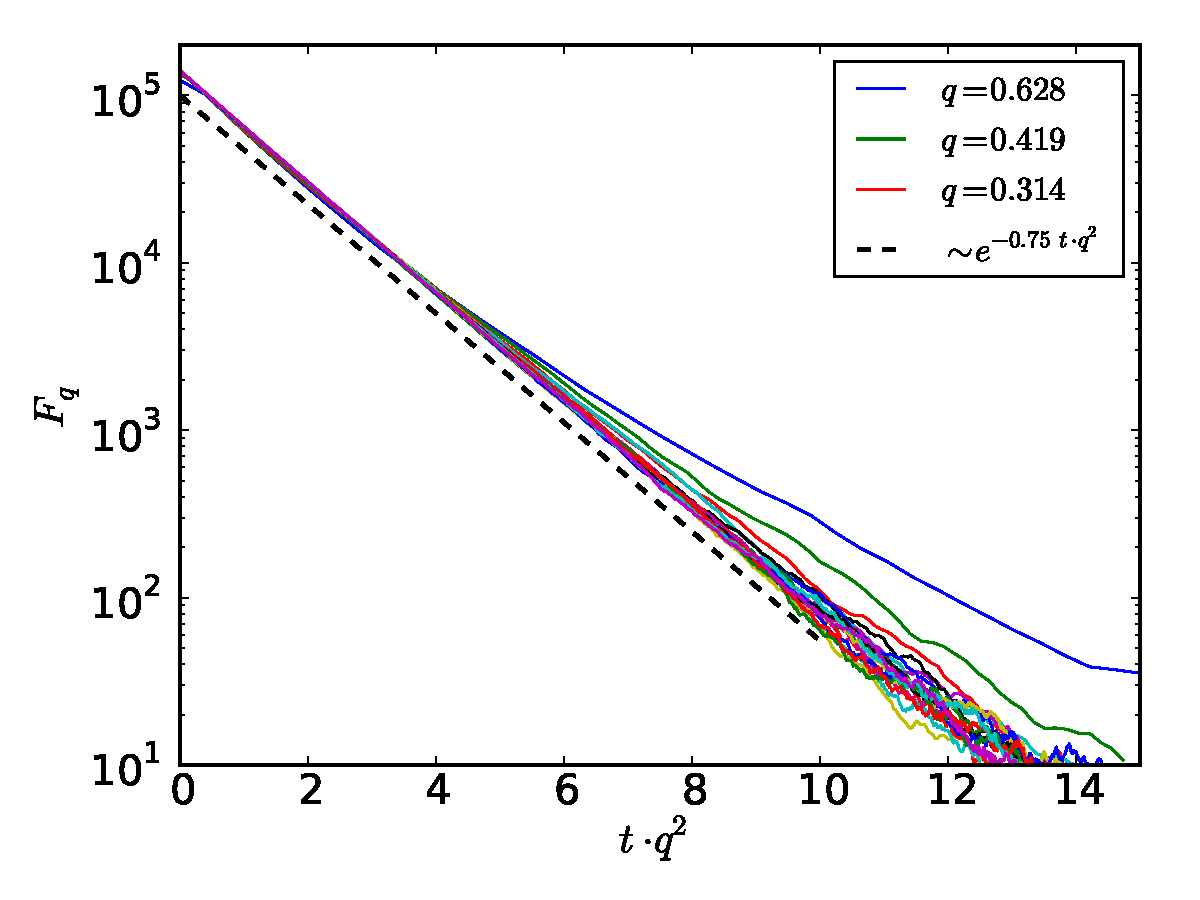
\includegraphics[width=0.65\textwidth]{../plot/relax_N10000000_010.pdf}
 \caption{Time dependence of the Fourier amplitudes $F_q$ for several values of $q$. The simulation used a time step $\Delta t=0.1$. For large values of $q\gtrsim0.2$, the relaxation of the Fourier amplitude is not purely exponential, but all values $q<0.1$ produced nice power-laws which overlap when using the time scaling $tq^2$.}
 \label{fig:relax_dt0.1}
\end{figure}

\begin{figure}[h]
 \centering
  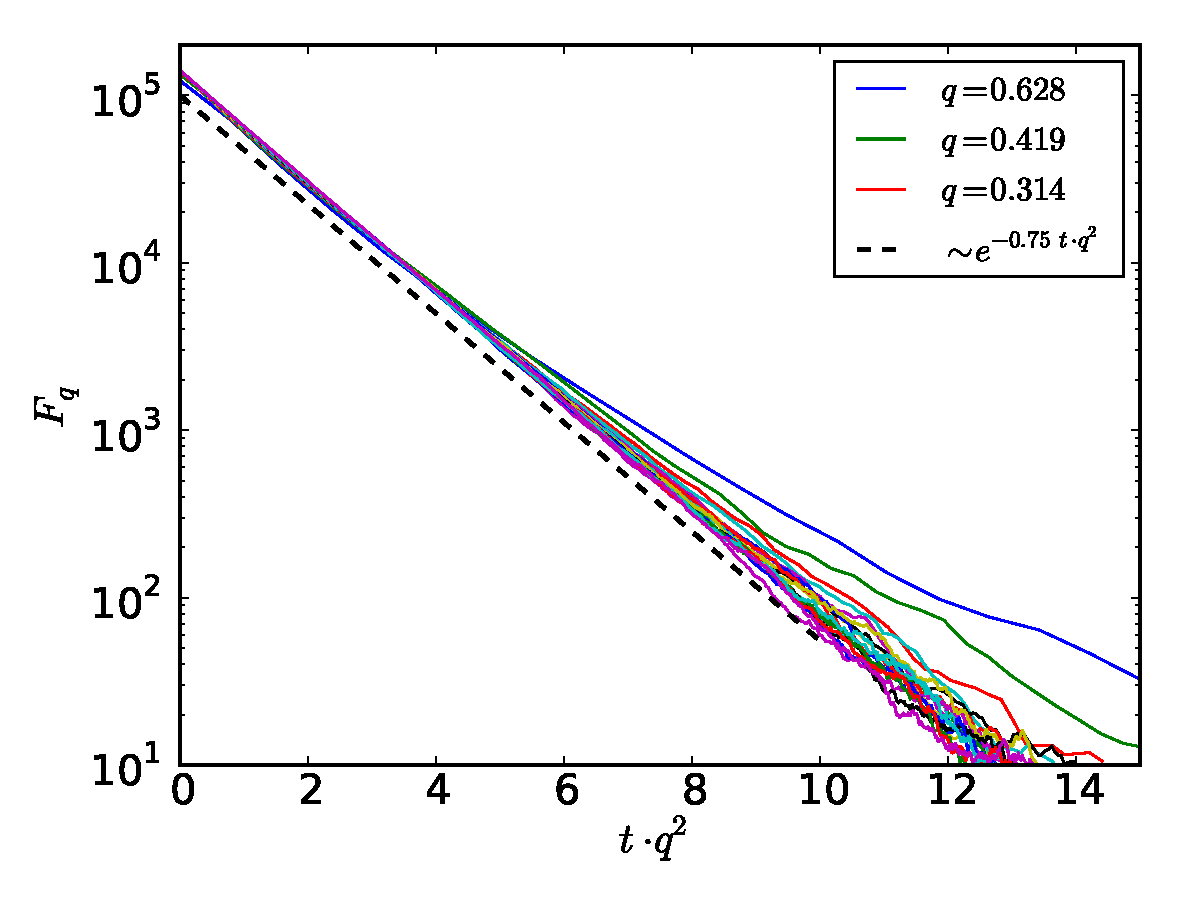
\includegraphics[width=0.65\textwidth]{../plot/relax_N10000000_020.pdf}
 \caption{The same as above, but with $\Delta t=0.2$.}
 \label{fig:relax_dt0.2}
\end{figure}

\begin{figure}[h]
 \centering
  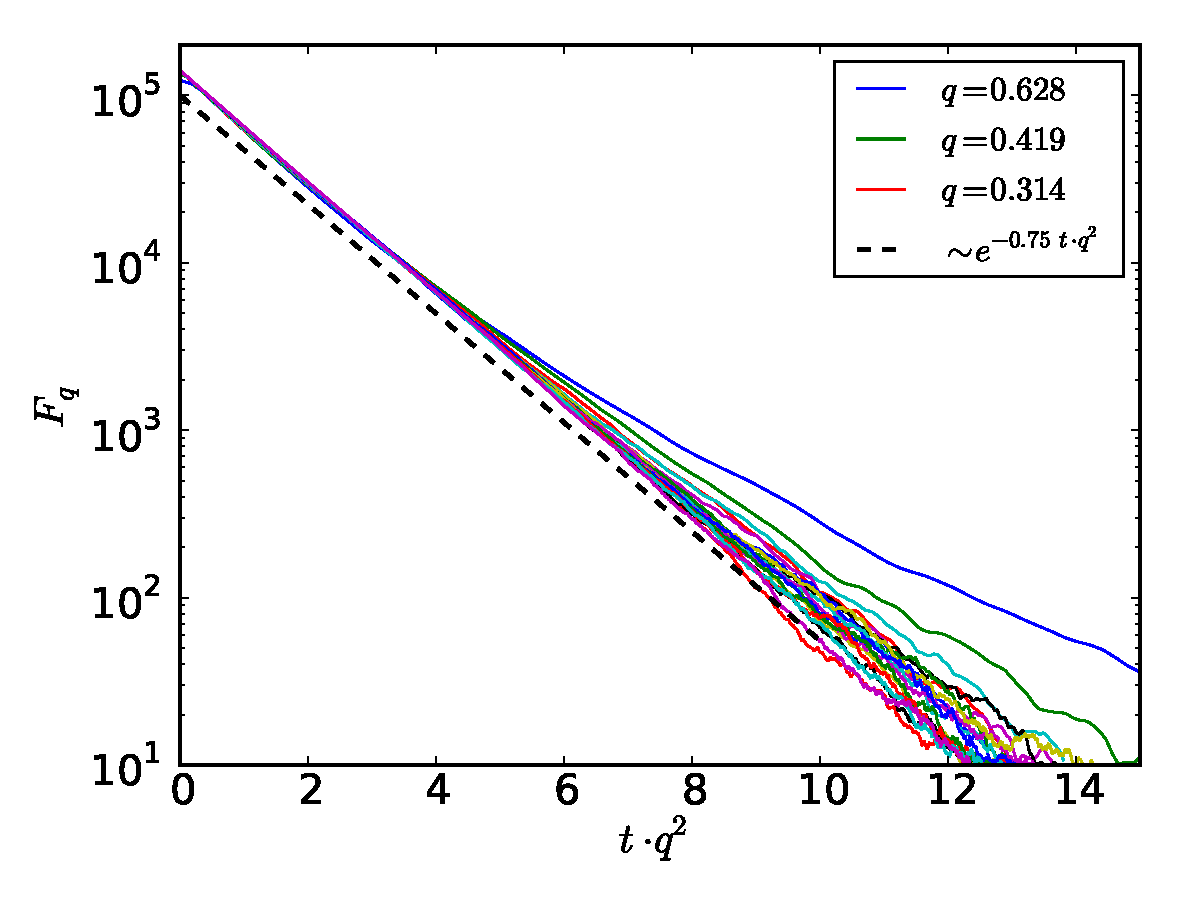
\includegraphics[width=0.65\textwidth]{../plot/relax_N10000000_005.pdf}
 \caption{The same as above, but with $\Delta t=0.05$.}
 \label{fig:relax_dt0.05}
\end{figure}

\end{document}